\chapter{Categorisation}
\label{chap:categorisation}

\section{Introduction}
\label{cat:sec:intro}

The basic experimental strategy for the observation of the \Hgg decay is to search for a resonance above a continuous \SM diphoton invariant mass spectrum. The sensitivity of this method is greatly enhanced by the categorisation of events by their expected mass resolution. Furthermore, it is possible to exploit additional particles in the detector to gain information about the likely process by which the Higgs boson was produced in each event, thus opening the possibility of making measurements of the rate of each production mode individually, as well as measurements of the strength of the Higgs boson's interaction with the individual particles involved in the different modes. These considerations motivate the following categorisation scheme. 

As was described in \Sec~\ref{sec:th:higgs_production_modes}, the Higgs boson is produced chiefly by four different production modes at the LHC. On the one hand, the most common, \ggH, produces a Higgs boson in isolation to first order, leading to just photons in the final state (ignoring the effect of \PU). On the other hand, the other production modes produce the Higgs boson in association with other particles. The \VBF production mode also has two quarks in the final state, which subsequently hadronize to form jets. The \VH production mode produces a Higgs boson in association to a \PW or \PZ boson, which subsequently decays to leptons or hadrons, sometimes involving missing energy if a neutrino was produced in the final state. Finally, the \ttH production mode produces the Higgs boson in association with two top quarks, which decay to bottom quarks and either hadrons or leptons. The additional particles produced in the final state of each mode give rise to a distinct signature which can be used to categorise events. For the two highest-rate modes, \ggH and \ttH, it is useful to take into account the expected mass resolution of the diphoton, which is obtained with a classification \BDT described in \Sec~\ref{cat:sec:dipho_bdt}. The categorisation of \VBF, \VH and \ttH events is then discussed in detail in \Sec\s~\ref{cat:sec:vbftag},~\ref{cat:sec:vhtag} and ~\ref{cat:sec:tthtag}.

\section{Diphoton BDT}
\label{cat:sec:dipho_bdt}

The classification of events by their expect mass resolution or signal-to-background ratio is obtained using a per-diphoton \BDT, which is hereafter referred to as \DiPhoBdt. The objective of the \DiPhoBdt is to separate signal-like diphotons (produced by the decay of a Higgs boson) from the \SM background diphotons, to assign a high output score to diphotons with a good mass resolution and where both individual photons have high \PhoIdBdt scores. 

Diphotons are produced by considering pairs of photons and their most likely primary vertex (as described in Chapter~\ref{chap:reconstruction}). Before the \DiPhoBdt is applied, the diphotons are required to satisfy the following requirements: both photons must pass a loose requirement on their \PhoIdBdt score, and the \pT of the leading (subleading) photon must be above $\mgg/3$ ($\mgg/4$).

The \DiPhoBdt is required to classify diphotons independently of the value of their invariant mass, otherwise the \mH value of the training sample would introduce a bias in the classification score. The input variables for the \DiPhoBdt are therefore required to be uncorrelated with the invariant mass of the diphoton system, and are listed below:

\begin{itemize}
\item the transverse momenta of both photons, divided by the invariant mass of the diphoton system to remove the correlation with \mH;
\item the $\eta$-position of both photons;
\item the \PhoIdBdt score of both photons;
\item the cosine of the opening angle between the photons in the $\phi$-direction;
\item the per-event estimated mass resolution of the diphoton, \sigmarv, assuming that the selected vertex is within 1\cm of the true vertex in the $z$-direction;
\item the per-event estimated mass resolution of the diphoton, \sigmawv, assuming that the selected vertex is more than 1\cm away from the true vertex in the $z$-direction;
\item the per-event estimate of the probability that the correct vertex was chosen, $p_{rv}$, obtained using the \VtxProbBdt described in \Sec~\ref{reco:sec:vtx_prob}.
\end{itemize}

The per-event estimated mass resolutions are obtained from the individual photon energy resolution estimates. The individual relative photon energy resolutions, labelled $\sigma^E_{\gamma_1}/E_{\gamma_1}$ and $\sigma^E_{\gamma_2}/E_{\gamma_2}$, are obtained from the semiparametric regression \PhoEnergyBdt as described in \Sec~\ref{sec:reco:photon:phoenergybdt}. Under the assumption that the selected vertex was within 1\cm of the true vertex, the dominant contribution to the uncertainty on the mass resolution is the energy resolution of each photon, and assuming Gaussian resolution functions, \sigmarv can be obtained by simply adding the individual relative photon energy resolutions in quadrature:
\begin{equation}
\sigmarv= \frac{1}{2} \sqrt{({\sigma^E_{\gamma_1}}/{E_{\gamma_1}})^2 +({\sigma^E_{\gamma_2}}/{E_{\gamma_2}})^2 }.
\end{equation} 
However, if the selected vertex was more than 1\cm away from the true one, the uncertainty on the opening angle contributes significantly to the mass resolution. The effect is modelled by including an additional term which represents the uncertainty on the mass due to the uncertainty on the vertex position, labelled $\sigma^V_{\gamma\gamma}$. The distance between the true vertex and the selected vertex follows a Gaussian distribution which has a width equal to the width of the beamspot multiplied by $\sqrt{2}$. Given the spatial positions of the photons, $\sigma^V_{\gamma\gamma}$ can therefore be calculated explicitly, and included in the sum in quadrature:
\begin{equation}
\sigmawv=  \sqrt{(\sigmarv)^2 +(\sigma^V_{\gamma\gamma}/\mgg)^2 }.
\end{equation} 

The \DiPhoBdt is trained on simulated sampled of signal and background processes. For the signal samples, events from different productions modes ($\mH=125\GeV$) are mixed according to their cross-section. The signal events used for training are also re-weighted by a factor $w$  given by 
\begin{equation}
w=  \frac{p_{rv}}{\sigmarv}+\frac{1-p_{rv}}{\sigmawv},
\end{equation} 
which codifies the fact that the signal-to-background ratio is inversely proportional to the mass resolution, and ensures that the \DiPhoBdt gives a high score to events with good mass resolution.
The background is composed of simulated diphotons originating from the irreducible and reducible \SM background processes. 

\Fig~\ref{fig:cat:diphobdt_a} shows the \DiPhoBdt output score for signal and background events in the range $100\GeV < \mgg < 180\GeV$, where a transformation is applied to flatten the signal distribution, so that the efficiency of a particular selection can be easily read. The \DiPhoBdt output score is validated using \Zee events in data and simulation, as can be seen on \Fig~\ref{fig:cat:diphobdt_b}.

\begin{figure}[h]
\centering
  \subfloat[]{
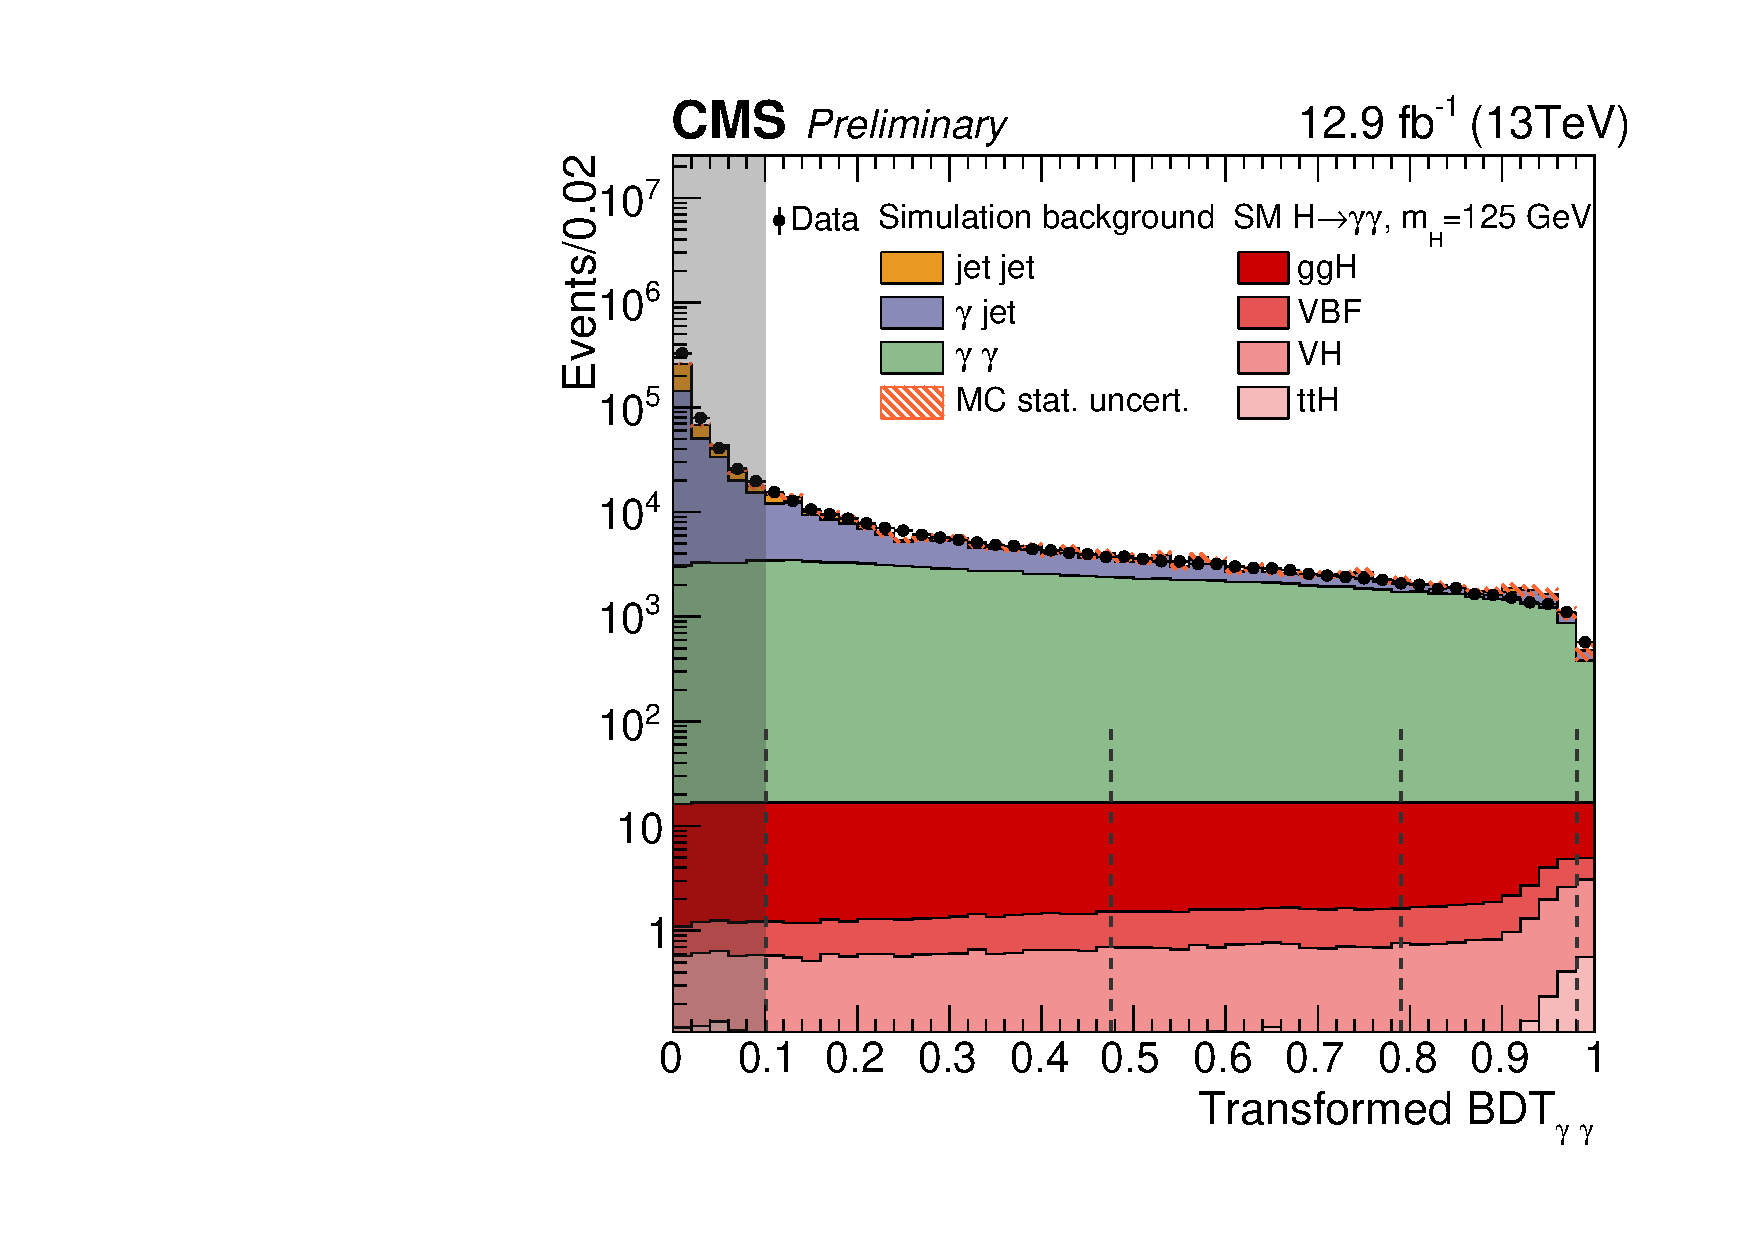
\includegraphics[width=0.45\textwidth]{catFigures/stack_scaled_resultFlat_mc_cat0_noratio.pdf}
\label{fig:cat:diphobdt_a}
}
  \subfloat[]{
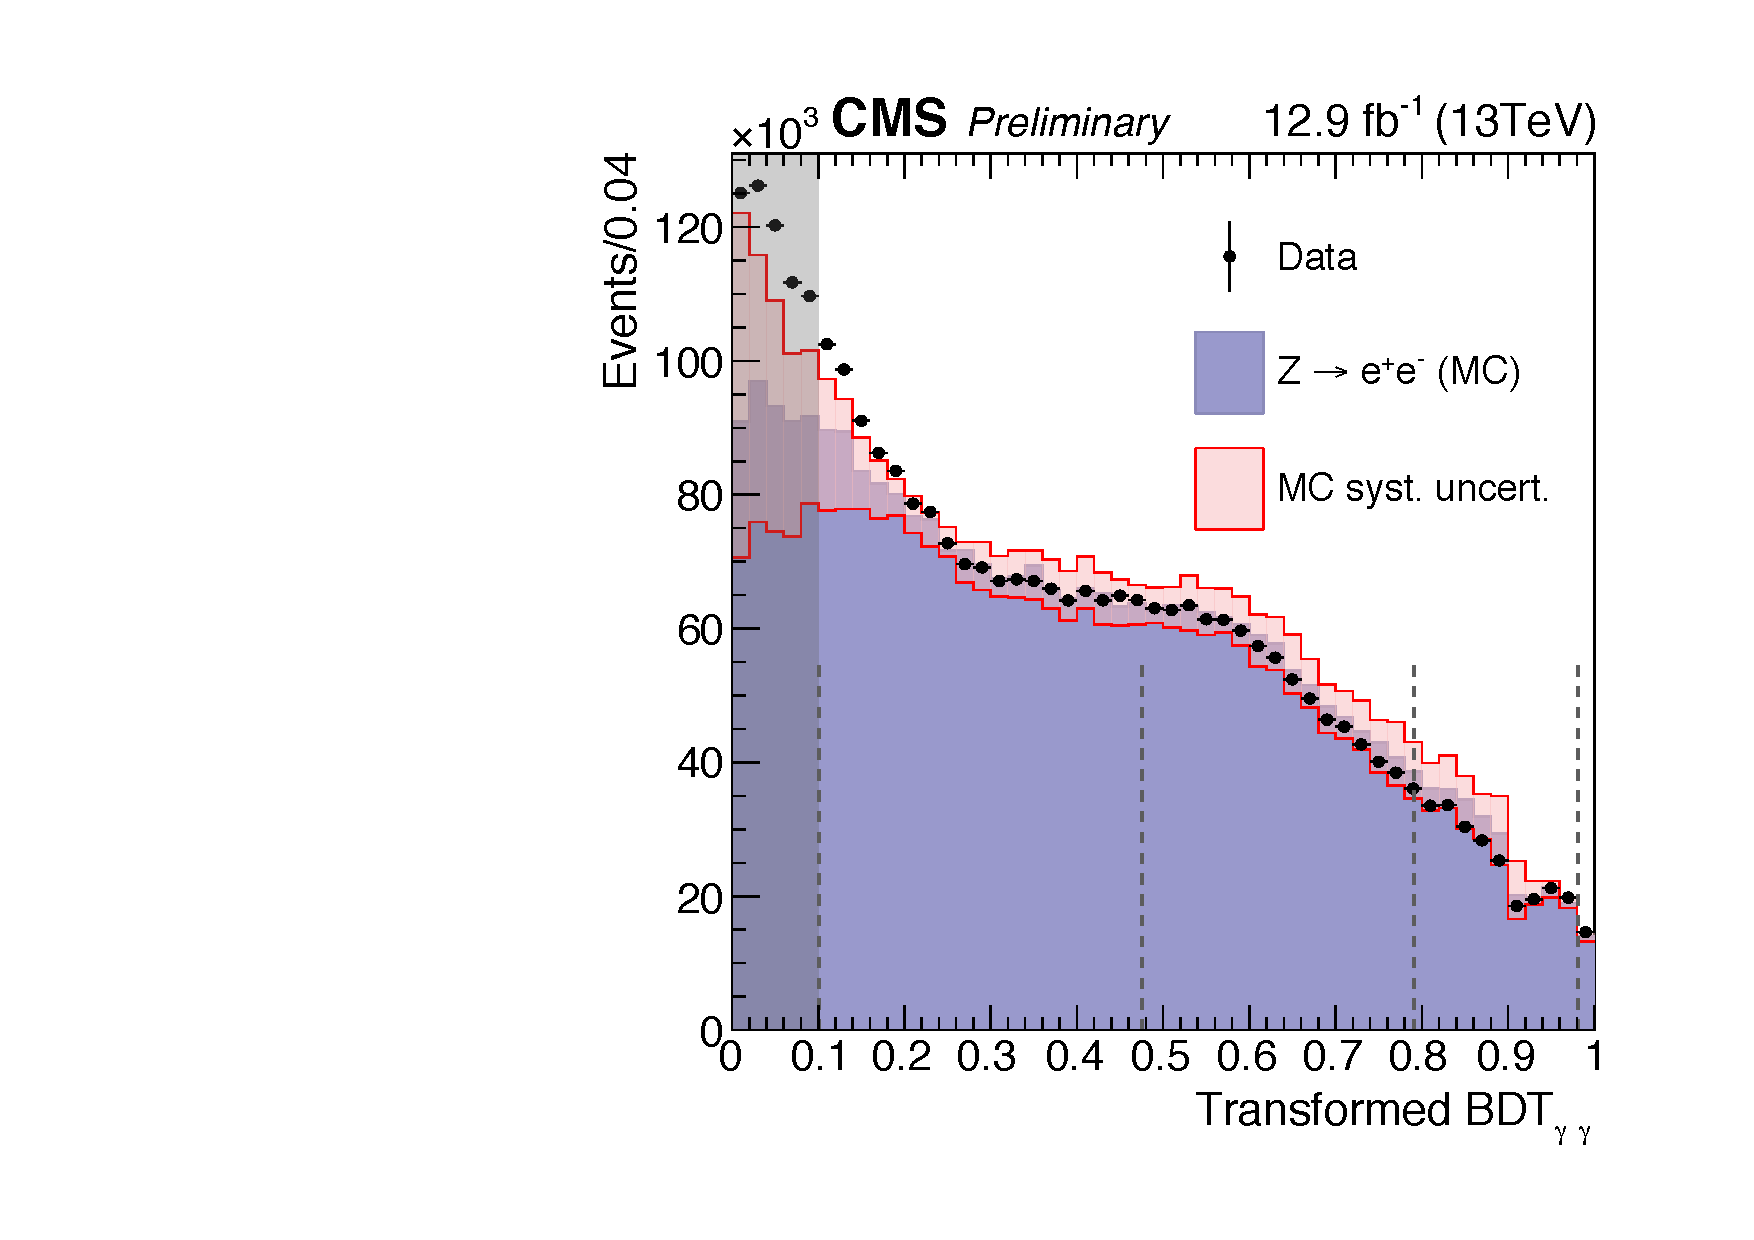
\includegraphics[width=0.45\textwidth]{catFigures/BDTTransfSyst_TrasfBDT_lin_1sigma_shiftPlusTransf_new_noratio.pdf}
\label{fig:cat:diphobdt_b}
}
\caption{ (a) The transformed \DiPhoBdt score for simulated signal and background events in the range $100\GeV < \mgg < 180\GeV$. The transformation flattens the signal distribution. (b) The transformed \DiPhoBdt score for \Zee events in data and simulation, where the electrons are reconstructed as photons. The pink shading represents the systematic uncertainty associated with the \PhoIdBdt and the \PhoEnergyBdt. For both (a) and (b), the vertical dashed lines represent the boundaries of the Untagged categories described in \Sec~\ref{cat:sec:untagged}, while the grey shading represents the area for which diphotons are rejected.}
\label{fig:cat:diphobdt}
\end{figure}

\section{\VBFTag categories }
\label{cat:sec:vbftag}

Higgs bosons in \CMS are produced chiefly via the \ggH production mode in the LHC environment. In this mode, the final state of the interaction involving the Higgs boson contains only the Higgs boson decay products to first order. Other production modes, by contrast, produce a Higgs boson in association with other particles. The additional particles can therefore be used to identify Higgs bososn events produced via \VBF, \VH or \ttH. The \VBF production mode has a cross-section approximately $10$ times smaller than that of \ggH. However, it produces the Higgs boson in association with two quarks, which result in two high-\pT jets when reconstructed. When studying teh \Hgg decay, the \VBF events therefore have a distinctive signature which aids in the indetification of such events. For this reason, although \VBF events are much less frequent than \ggH events, the most sensitive \VBFTag category has a signal-to-background ratio comaprable to the most sensitive category in the analysis. Including \VBFTag categories in the analysis therefore significantly improves the overall sensitivity of the analysis.



The \VBFTag categories are obtained by first identifying events which contain two high-\pT jets, collectively referred to as a \emph{dijet}. For each diphoton candidate, the individual jets are obtained as described in \Sec~\ref{reco:sec:jets} after \PFCHS with respect to the vertex selected in \Sec~\ref{reco:sec:vertex} is applied. Candidate \VBFTag events are required to have at least two jets which pass the \PU removal requirements and are separated by \PF photon candidates by $\Delta R = 0.5$. The leading (subleading) jet, i.e~the one with the highest \pT (second-highest \pT) in the event, is required to satisfy $\pT > 30 \GeV$ ($\pT > 20 \GeV$). For events passing these requirements, and additional requirement on the invariant mass of the dijet composed of the leading and subleading jets (\mjj) is imposed: $\mgg > 250\GeV$. Events which pass all of the above are said to pass the \emph{dijet preselection}.

For events passing the dijet preselection, the \VBFTag categorisation proceeds as follows. First, a per-event \BDT is used to identify \VBF-like dijets, which is hereafter referred to as \DiJetBdt. The \DiJetBdt is trained to treat simulated \VBF events as signal, and to treat simulated \ggH events (where dijets are formed from \PU or initial or final state radiation) and \SM processes which produce jets as background. The \DiJetBdt does not have any information about the quality and mass resolution of the photons in the diphotons int he event, so a further per-event \BDT is used to recover this information, referred to as the \DiPhoDiJetBdt. The \DiPhoDiJetBdt has amongst its inputs the scores from the \DiPhoBdt and the \DiJetBdt, and thus is able to combine the \VBF-like dijet identification power of one \BDT with with mass resolution information from the other. In the  \DiPhoDiJetBdt, \ggH events cannot be treated as background since the \DiPhoBdt would not be well-behaved. So \ggH events are treated as neither signal nor background which training the \DiPhoDiJetBdt. A selection on the output score of the \DiPhoDiJetBdt is then used to select events fro the \VBFTag categories.

The \DiJetBdt is designed to use the kinematic properties of the diphoton-dijet system to identify \VBF-like events where the Higgs boson decayed via \Hgg. It is trained on simulated samples of diphoton events where the signal is defined \VBF (\Hgg) events where $\mH=125\GeV$ and the background consists of \SM events with a diphoton and a dijet in the final state, and in addition a simulated sample of \ggH events with $\mH=125\GeV$. The input variables for this \BDT are listed below:
\begin{itemize}
\item the invariant-mass scaled transverse momentum ($\pT/\mgg$) for the leading and subleading photons in the diphoton candidate;
\item the transverse momenta of the leading and subleading jets in the dijet;
\item the invariant mass of the dijet \mjj;
\item the separation of the jets in the dijet in the $\eta$-direction ($|\eta_{j_1} - \eta_{j_2}$);
\item the \emph{Zeppenfeld} variable~\cite{Zeppenfeld}, $\eta^{*} = \eta_{\gamma_1+\gamma_2} - \eta_{j_1}/2 - \eta_{j_2}/2$, where $\eta_{\gamma_1+\gamma_2}$ is the position in $\eta$ of the vector sum of the photon directions;
\item the separation in the $\phi$-direction between the dijet and the diphoton.
\end{itemize}

The \DiPhoDiJetBdt is designed to re-introduce information about the sensitivity of signal events while maintaining the power to identify \VBF-like events. This is obtained by training the \BDT on simulated events where the signal is a sample of \VBF \Hgg events with $\mH=125\GeV$, while the background is composed of the standard simulated diphoton background, as for teh \DiJetBdt training. In this case, \ggH events are treated as neither signal nor background. The inputs to the \BDT are the following:
\begin{itemize}
\item the output score of the \DiPhoBdt;
\item the output score of the \DiJetBdt;
\item the invariant mass-scaled \pT of the diphoton system, which is included since it has a significant correlation to both the other inputs.
\end{itemize}

Selections on the \DiPhoDiJetBdt output score are used to define two \VBFTag categories. The most sensitive category is referred to as \VBFTag 0 and contains all the events with the highest \DiPhoDiJetBdt output score above some boundary. Another, less sensitive category named \VBFTag 1 contains all events for which the  \DiPhoDiJetBdt output score  is below the first boundary, but still above a second boundary. Events for which the \DiPhoDiJetBdt output score is below the second boundary fail the \VBFTag categorisation, but may still be considered for inclusion in other analysis event categories, such as the Untagged categories described in \Sec~\ref{cat:sec:untagged}. The location of the two boundaries is optimised first by maximising the value of the signal-to-background ratio in the \VBFTag 0 category, and then repeating the procedure after fixing the first boundary to maximise the signal-to-background ratio in the \VBFTag 1 category. Of the simulated signal events which are categorised as \VBF-like, the \VBFTag 0 category contains approximately 72\% \VBF events and 27\% \ggH events, and the  \VBFTag 1 category contains approximately 55\% \VBF events and 43\% \ggH events. 

The distributions of the output score of the \DiJetBdt for the different simulated production modes are shown in \Fig~\ref{fig:cat:dijetbdt_sig} and comparing data and simulated background ( and some simulate signal) events in \Fig~\ref{fig:cat:dijetbdt_all}. The analogous distributions for the \DiPhoDiJetBdt output score are shown in \Fig~\ref{fig:cat:diphodijetbdt_sig} \Fig~\ref{fig:cat:diphodijetbdt_all} respectively.

\begin{figure}[h]
\centering
  \subfloat[\DiJetBdt output by production mode]{
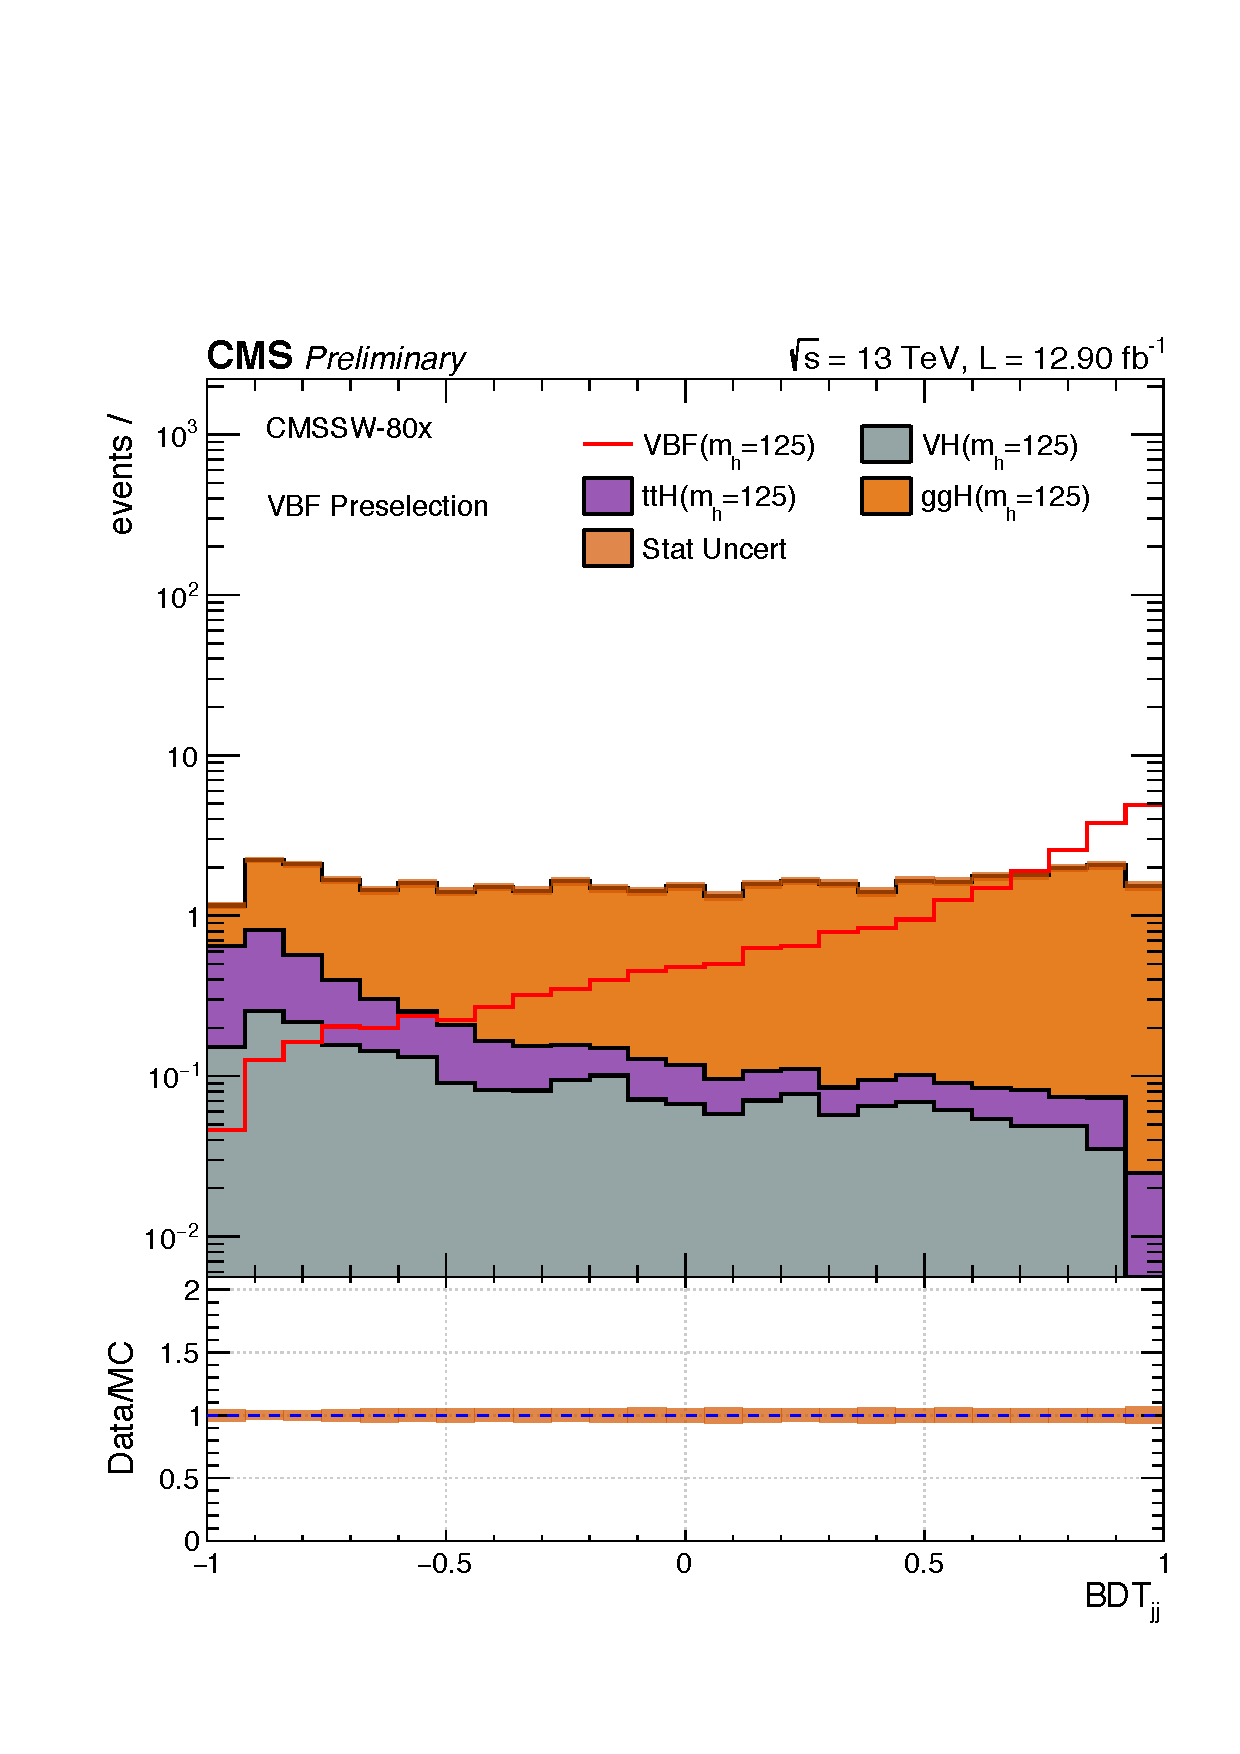
\includegraphics[width=0.45\textwidth]{catFigures/stack_histogram_dijet_mva_signal_14-07-2016_.pdf}
\label{fig:cat:dijetbdt_sig}
}
  \subfloat[\DiJetBdt output comparing data and simulated signal and background]{
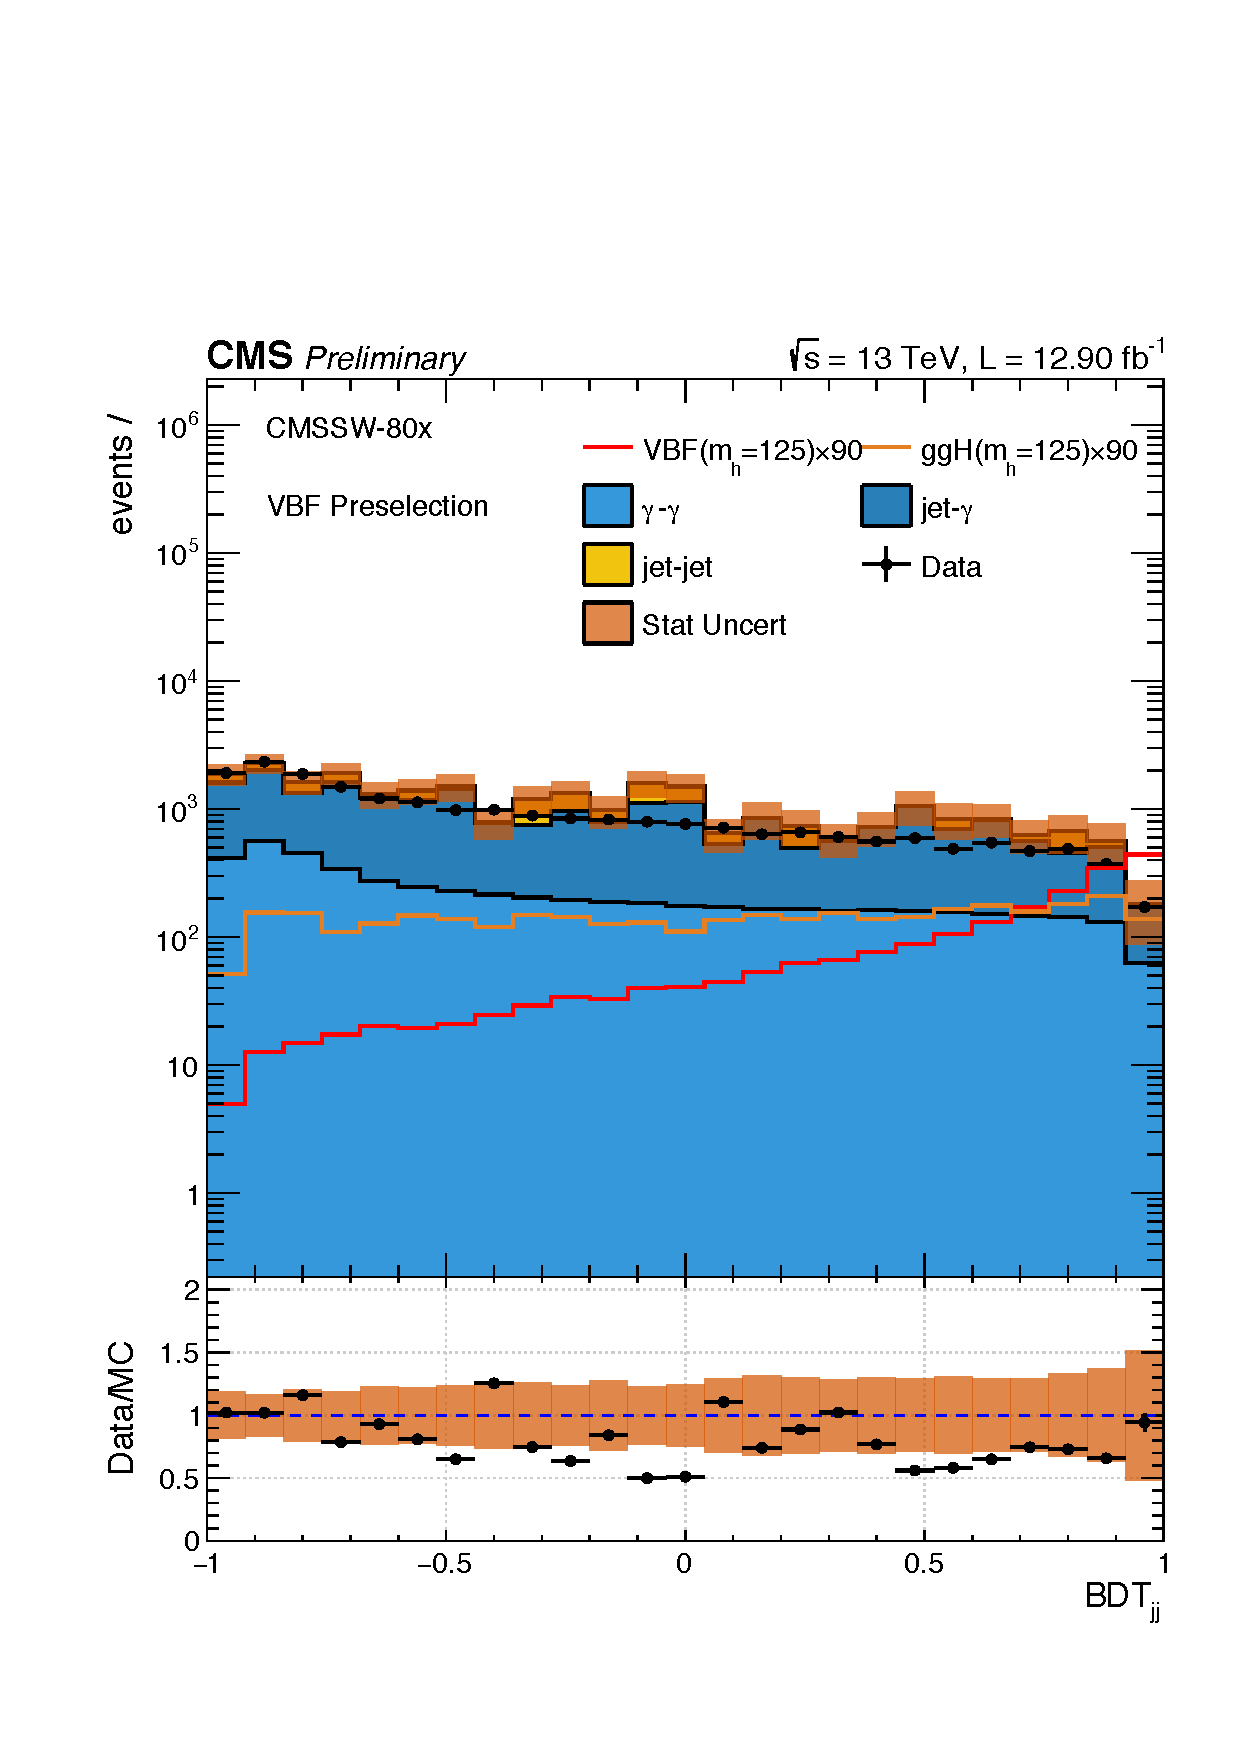
\includegraphics[width=0.45\textwidth]{catFigures/stack_histogram_dijet_mva_VBF_14-07-2016_.pdf}
\label{fig:cat:dijetbdt_all}
}
\\
  \subfloat[\DiPhoDiJetBdt output by production mode]{
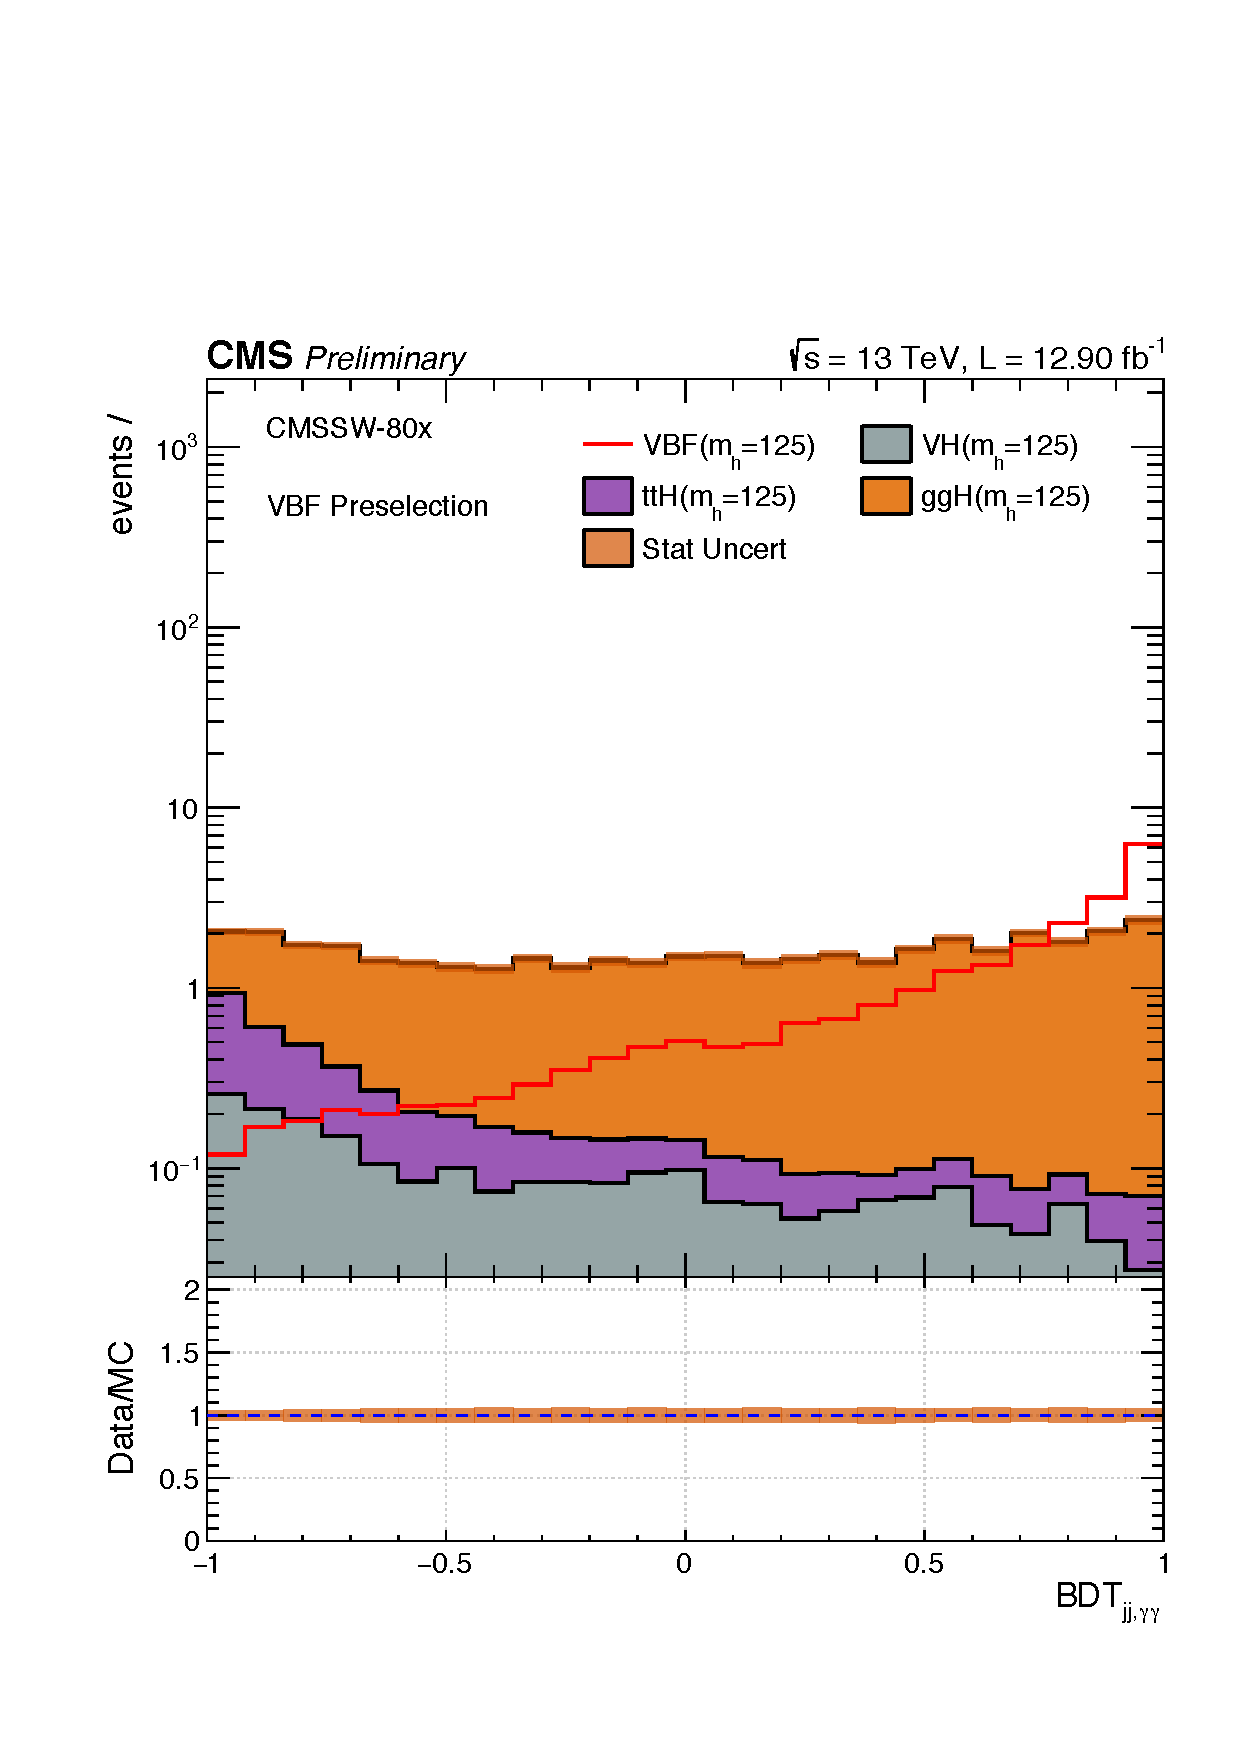
\includegraphics[width=0.45\textwidth]{catFigures/stack_histogram_dipho_dijet_MVA_signal_14-07-2016_.pdf}
\label{fig:cat:diphodijetbdt_sig}
}
  \subfloat[\DiPhoDiJetBdt output comparing data and simulated signal and background]{
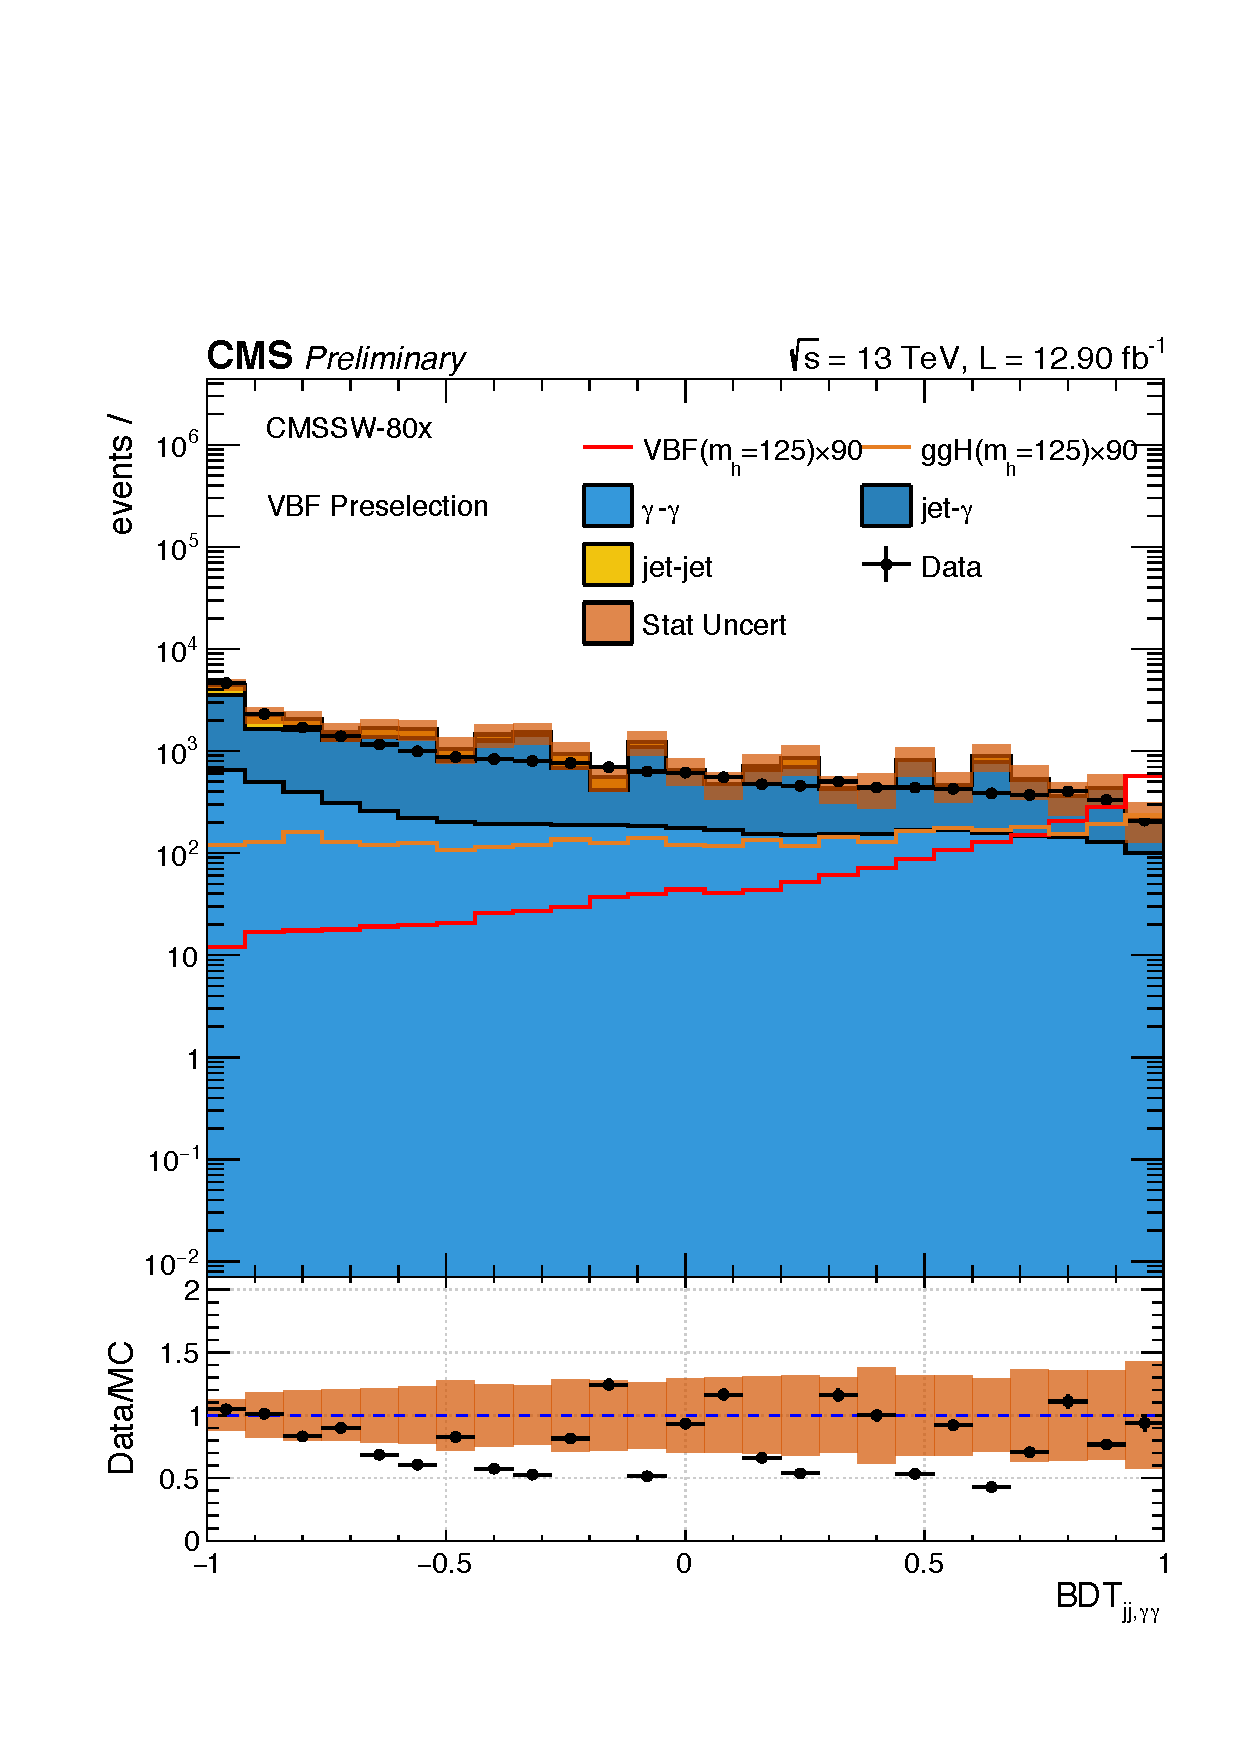
\includegraphics[width=0.45\textwidth]{catFigures/stack_histogram_dipho_dijet_MVA_VBF_14-07-2016_.pdf}
\label{fig:cat:diphodijetbdt_all}
}
\caption{The output scores of the \DiJetBdt and \DiPhoDiJetBdt split by simulated production mode and comparing data and simulated signal and background.}
\label{fig:cat:vbf_bdts}
\end{figure}

\section{VH-Tagged categories}
\label{cat:sec:vhtag}
\subsection{Tight and loose VH-Tagged categories}
\subsection{Missing energy VH-Tagged categories}

\section{\TTHTag categories}
\label{cat:sec:tthtag}

Higgs boson events are produced in association with a pair of top quarks in the \ttH mode. The final state therefore contains two photons from the Higgs boson decay, as well as two $\Pbottom$ quarks and decay products from two $\PW$ bosons. The $\PW$ bosons will decay either hadronically (to quarks, which subsequently hadronize to form jets) or leptonically (to a lepton and corresponding neutrino). The signatures of these events can be used to identify Higgs boson events likely to have been produced by the \ttH mechanism. The cross-section of \ttH production is low, so the benefit to the analysis in terms of final significance of an observation is small. However, the categorisation of \ttH-like events is important because it allows the measurement of the strength of the interaction of the Higgs boson with top quarks. Various extensions to the \SM predict enhanced values of the strength of the \ttH interaction, and such models can be tested through the experimental measurement of the cross-section of \ttH events decaying to \Hgg.

Two \TTHTag exclusive categories are defined in this analysis. On the one hand, the \TTHLeptonicTag category aims to select \ttH events where at least one of the $\PW$ bosons decayed leptonically. On the other hand, the \TTHHadronicTag category targets events where both $\PW$ bosons decayed to quarks. The selections for each of these categories are defined separately and are described below.

The \TTHLeptonicTag 


\section{Untagged categories}
\label{cat:sec:untagged}

Diphotons which are not categorised into the \VBF-tagged, \VH-tagged or \ttH-tagged categories can still be included in the inclusive categories, which are labelled as \emph{Untagged}. Since \ggH events are produced without any additional particles to first order, they are typically placed in the Untagged categories. Events which are included in the Untagged can be split into subcategories to improve the overall sensitivity of the analysis. The splitting is performed by defining boundaries in the \DiPhoBdt output score distribution. The location of the boundaries as well as the number of subcategories is optimised using simulated signal and background samples which are independent from those used to train the \DiPhoBdt.

For a given number of subcategories $N_\text{subcat}$, the boundaries are spaced evenly throughout the \DiPhoBdt output score distribution.  For events each subcategory. Events falling in the subcategory below the lowest boundary are discarded.  Simplified models are used to parametrise the signal and background \mgg distributions in the remaining categories. For the signal, the model is a sum of two Gaussian functions, which model the detector resolution and the uncertainty due to incorrect vertex assignment respectively. For the background, the \mgg spectrum is modelled using an exponential shape. The expected significance is then obtained by producing an Asimov dataset~\cite{Cowan:2010js} from the signal and background models in each category, and then performing a simultaneous signal and background fit. This procedure is iteratively repeated, allowing the boundaries between the subcategories to float, maximizing the expected significance.

The procedure can be repeated separately for arbitrary values of $N_\text{subcat}$. In this analysis, $N_\text{subcat}=4$ was chosen (ignoring the subcategory below the lowest boundary), as moving to $N_\text{subcat}=5$ produced a negligible improvement in the expected significance. The boundaries extracted from this optimisation procedure are represented by the vertical dashed lines in \Fig\s~\ref{fig:cat:diphobdt_a} and~\ref{fig:cat:diphobdt_b}. The resulting Untagged categories are numbered from Untagged 0 (most sensitive) to Untagged 3 (least sensitive), and diphotons which have a \DiPhoBdt score too low to enter Untagged 3 are discarded.


